\chapter{Recapitulare examen}

\section{Model 1}

\indent\indent 1. Fie spațiul vectorial:
\[
  V = \{ p \in \RR_2[X] \mid p'(1) = 0 \}.
\]
\begin{enumerate}[(a)]
\item Găsiți complementul său ortogonal $ V^\perp $.
\item Găsiți o bază ortonormată în $ V \oplus V^\perp $.
\end{enumerate}

\emph{Indicații:} (a) $ V = \{ aX^2 + bX + c \mid 2a + b = 0 \} $, deci
$ \dim V = 2 \Rightarrow \dim V^\perp = 1 $.

(b) Se ia reuniunea bazelor din $ V $ și $ V^\perp $, care este o bază
a sumei directe. Se aplică Gram-Schmidt pentru aceasta.
\vspace{1cm}

2. Aduceți la forma canonică și desenați conica:
\[
  x^2 - 4xy + 4y^2 - 6x + 2y + 1 = 0.
\]

\emph{Răspuns:} Conica este o parabolă:
\begin{center}
  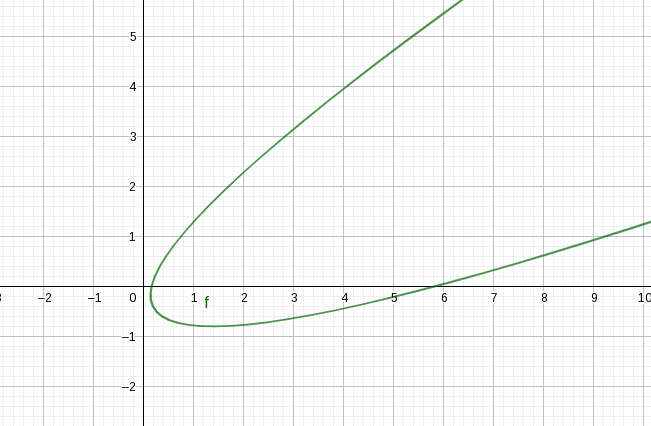
\includegraphics[scale=0.5]{figs/parabola12.png}
\end{center}

\vspace{1cm}

3. Rezolvați ecuațiile diferențiale:
\begin{enumerate}[(a)]
\item $ (x + y - 2) dx + (x + y) dy = 0 $; \hfill{(ecuație exactă)}
\item $ xy' = y + x^2 y^2, x > 0 $. \hfill{(ecuație Riccati)}
\end{enumerate}

\vspace{1cm}

4. Rezolvați sistemul diferențial:
\[
  \begin{cases}
    x' &= y + z \\
    y' &= x + z \\
    z' &= x + y
  \end{cases}
\]
cu condițiile inițiale $ x(0) = -1, y(0) = 0, z(0) = 0 $.

\emph{Indicație:} Se aduce matricea sistemului la forma canonică Jordan:
(matricea este chiar diagonalizabilă):
\[
  A = \begin{pmatrix}
    0 & 1 & 1 \\
    1 & 0 & 1 \\
    1 & 1 & 0
  \end{pmatrix} \Rightarrow J =
  \begin{pmatrix}
    -1 & 0 & 0 \\
    0 & -1 & 0 \\
    0 & 0 & 2
  \end{pmatrix},
\]
apoi se calculează $ e^{At} $ folosind această formă simplificată.

%%%%%%%%%%%%%%%%%%%%%%%%%%%%%%%%%%%%%%%%%%%%%%%%%%%%%%%%%%%%%%%%%%%%%%

\section{Model 2}

\indent\indent Fie spațiul vectorial:
\[
  V = \{(x, y, z, t) \in \RR^4 \mid x + y - 2z + t = 0 \}.
\]
\begin{enumerate}[(a)]
\item Găsiți complementul ortogonal, $ V^\perp $;
\item Găsiți o bază ortonormată în $ V $.
\end{enumerate}

\emph{Indicație:} $ \dim V = 3 $, deci $ \dim V^\perp = 1 $.
Avem:
\[
  V = \{(-\alpha + 2\beta - \gamma, \alpha, \beta, \gamma) \in \RR^4 \} = %
  \dr{Sp} \{(-1, 1, 0, 0), (2, 0, 1, 0), (-1, 0, 0, 1) \}
\]
și se alege $ V = \dr{Sp}\{(a, b, c, d)\} $ astfel încît
\[
  \langle (a, b, c, d), v \rangle = 0,
\]
unde $ v $ este, pe rînd, fiecare vector din baza lui $ V $.

\vspace{1cm}

2. Aduceți la forma canonică și reprezentați conica:
\[
  x^2 - 2xy + 3y^2 - 4x + 6y - 4 = 0.
\]

\emph{Răspuns:} Conica este o elipsă:
\begin{center}
  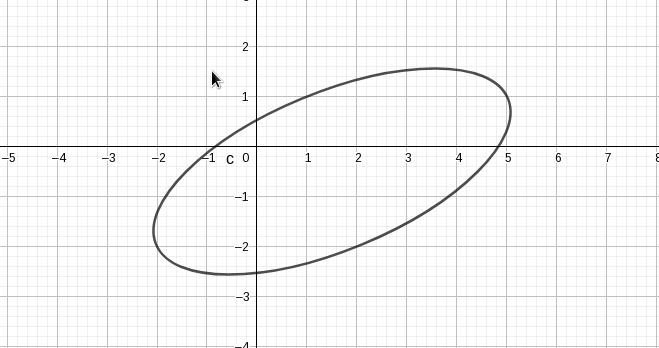
\includegraphics[scale=0.5]{figs/elipsa22.png}
\end{center}

\vspace{1cm}

3. Rezolvați ecuațiile diferențiale:
\begin{enumerate}[(a)]
\item $ y' + y\sin x = -\sin x \cos x $; \hfill{(ecuație liniară și neomogenă)}
\item $ (3x^2 - y) + (3y^2 - x) y' = 0 $. \hfill{(ecuație exactă)}
\end{enumerate}

\vspace{1cm}

4. Rezolvați sistemul diferențial:
\[
  \begin{cases}
    x' &= x - y \\
    y' &= -4x + y
  \end{cases},
\]
cu condițiile inițiale $ x(0) = 1, y(0) = -1 $.

\emph{Indicație:} Se poate folosi forma Jordan pentru matricea sistemului sau
se pot aplica metodele din \S\ref{sec:sist-ct}, deoarece matricea este diagonalizabilă
și este $ 2 \times 2 $.

%%%%%%%%%%%%%%%%%%%%%%%%%%%%%%%%%%%%%%%%%%%%%%%%%%%%%%%%%%%%%%%%%%%%%%

\section{Model 3}

\indent\indent 1. Fie spațiul vectorial:
\[
  V = \{ M \in M_2(\RR) \mid M = M^t \}.
\]
\begin{enumerate}[(a)]
\item Găsiți complementul ortogonal al lui $ V $;
\item Găsiți o bază ortonormată în $ V $.
\end{enumerate}

\emph{Indicații:} Matricele din $ V $ au elementele egale
pe diagonala secundară, deci $ \dim V = 3 $. Rezultă $ \dim V^\perp = 1 $,
adică $ V^\perp = \dr{Sp} \Big\{ \begin{pmatrix} a & b \\ c & d \end{pmatrix} \Big\} $,
care să fie perpendiculară pe cele 3 matrice din baza lui $ V $.

\vspace{1cm}

2. Aduceți la forma canonică și reprezentați conica:
\[
  4xy - 3y^2 + 4x - 14y - 7 = 0.
\]

\emph{Răspuns:} Conica este o hiperbolă:
\begin{center}
  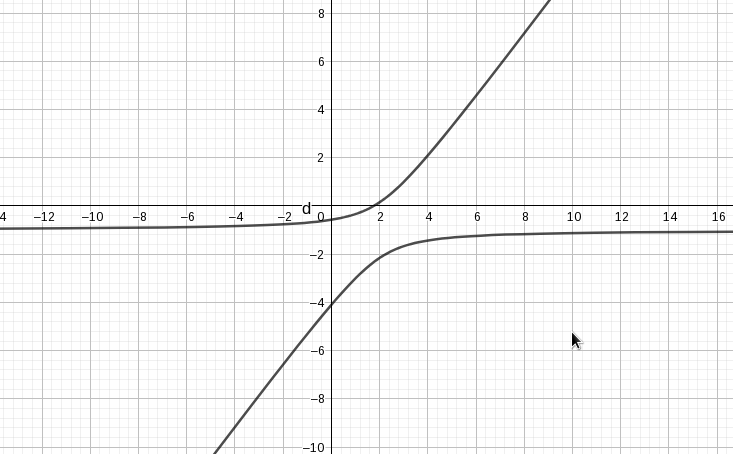
\includegraphics[scale=0.5]{figs/hiperbola32.png}
\end{center}

\vspace{1cm}

3. Rezolvați ecuațiile diferențiale:
\begin{enumerate}[(a)]
\item $ (1 - x^2y) + x^2(y - x)y' = 0 $; \hfill{(factor integrant $ \mu = \mu(x) $)}
\item $ y = xy' - {y'}^2 $. \hfill{(ecuație Lagrange)}
\end{enumerate}

\vspace{1cm}

4. Fie matricea:
\[
  A = \begin{pmatrix}
    1 & -1 & 1 \\
    1 & 1 & -1 \\
    0 & -1 & 2 
  \end{pmatrix}
\]
\begin{enumerate}[(a)]
\item Să se calculeze $e^{At}$, pentru $t \in \RR$;
\item Să se determine soluția generală a sistemului $X' = AX$, apoi soluția particulară
  care verifică condiția $x(0) = 1, y(0) = 2, z(0) = 0$.
\end{enumerate}

\emph{Indicație:} Vezi \S\ref{sec:jordan} (completați detaliile lipsă din rezolvare).


%%% Local Variables:
%%% mode: latex
%%% TeX-master: "../ag-18-19"
%%% End:
